\documentclass[10pt]{beamer}
\setbeamertemplate{caption}[numbered]
\usetheme{Malmoe}

\usepackage[utf8]{inputenc}
\usepackage[T1]{fontenc}
\usepackage[english ]{babel}

\usepackage{amsmath}

\usepackage{graphicx}
\usepackage{wrapfig}

\usepackage{multimedia}

\usepackage{stmaryrd}
\usepackage{bbm}
\usepackage{listings}
\usepackage[section]{placeins}
\usepackage{caption}
\usepackage{url}

\usepackage{color} %red, green, blue, yellow, cyan, magenta, black, white
\definecolor{mygreen}{RGB}{28,140,0} % color values Red, Green, Blue
\definecolor{mylilas}{RGB}{170,55,241}

\lstset{language=Matlab,%
    %basicstyle=\color{red},
    basicstyle=\footnotesize\ttfamily,
    breaklines=true,%
    morekeywords={matlab2tikz},
    keywordstyle=\color{blue},%
    morekeywords=[2]{1}, keywordstyle=[2]{\color{black}},
    identifierstyle=\color{black},%
    stringstyle=\color{mylilas},
    commentstyle=\color{mygreen},%
    showstringspaces=false,%without this there will be a symbol in the places where there is a space
    numbers=left,%
    numberstyle={\tiny \color{black}},% size of the numbers
    numbersep=9pt, % this defines how far the numbers are from the text
    emph=[1]{for,end,break},emphstyle=[1]\color{red}, %some words to emphasise
    %emph=[2]{word1,word2}, emphstyle=[2]{style},    
    frame= single,
}

\title{Programming Pentago with Matlab}
\author{Gustavo C. PINTON and Marcelo M. F. DE CARVALHO}
\institute{ 
\includegraphics[scale=0.3]{images/LogoSupelec}}
\date{2015}

\addtobeamertemplate{navigation symbols}{}{
    \usebeamerfont{footline}%
    \usebeamercolor[fg]{footline}%
    \hspace{1em}%
    \insertframenumber/\inserttotalframenumber
}
\setbeamercolor{footline}{fg=blue}
\setbeamerfont{footline}{series=\bfseries}

\begin{document}

\begin{frame}
\titlepage
\end{frame}

\begin{frame}
\frametitle{Contents }
\tableofcontents
\end{frame}

\section{Introduction}

\begin{frame} 

\frametitle{Introduction}
\framesubtitle{The Objective}


	\begin{itemize}
	  
		\item To implement an artificial intelligence able to play effectively the
		board game Pentago.
		\item To use Matlab to achieve so
			\begin{itemize}
			  \item Most are developed in C++... BUT Matlab has a pedagogical value.
			  
			  \begin{itemize}
			  	\item Previously used at Supélec's EL.
			  	\item Previously used by our advisor to implement an AI
			  \end{itemize}
			  
			\end{itemize}

	\end{itemize}


\end{frame}

\begin{frame}
\frametitle{Introduction}
\framesubtitle{What is Pentago?}

	\begin{itemize}
	  
		\item Two-player game introduced by Tomas Flodén in 2005
		\item How do we play it?
			\begin{itemize}
			  
			  \item We play it using a 6x6 board divided into four 3x3 sub-boards (or
			  quadrants).

			  \item Each player assumes a color (a white player, a black player). 
			  Taking turns, each one places a marble of his color onto an unoccupied
			  space on the board, and then rotate one of the sub-boards by 90 degrees,
			  either clockwise or anti-clockwise.

			  \item A player wins by getting five of their marbles in a vertical,
			  horizontal or diagonal row.

			  \item If all 36 spaces on the board are occupied without a row of five
			  being formed then the game is a draw.
			  
			\end{itemize}

	\end{itemize}
\end{frame}

\begin{frame}
\frametitle{Introduction}
\framesubtitle{Why Pentago? }

	\begin{itemize}
	  
		\item Two player, deterministic, perfect knowledge, zero sum game.
		
			\begin{itemize}
			  \item Interesting for computer science:
			  		\begin{itemize}
			  		  \item  AI development and theoretical complexity analysis.
			  		\end{itemize}
			  \item Great popularity worldwide:
			  		\begin{itemize}
			  		  \item Pentago: smaller number of state and some symmetries.
			  		  \item Less complex.
			  		\end{itemize} 
			\end{itemize}
			
		\item Pentago has been strongly solved with a Cray supercomputer at NERSC.
		
			\begin{itemize}
			  
			  \item How far can we go using Matlab and a regular laptop?

			  \item Would it be suitable for Human x Machine and Machine x Machine
			  battles?
			  
			\end{itemize}

	\end{itemize}
\end{frame}

\begin{frame}
\frametitle{Introduction}
\framesubtitle{Work Planning}

	\begin{itemize}
	  
		\item First, Pentago structure (i.e. player vs player enabled).
		
			\begin{itemize}
			  \item Graphical interface.
			  \item Allow piece placing in an empty space and turn structure.
			  \item Introduce rotation.
			  \item Introduction of a «game over» clause (win or tie).		  		 
			\end{itemize}
			
		\item Second, artificial intelligence (i.e. player vs AI enabled)
		
			\begin{itemize}
			  
			  \item Random play AI.

			  \item Research about possible solving algorithms.
			  
			\end{itemize}
		
		\item Finally, AI optimizing (i.e. AI vs AI enabled)
		
			\begin{itemize}
			  
			  \item Implementation of efficient solving algorithms.
			  \item Further tuning for optimal results.
			  
			\end{itemize}
		
	\end{itemize}
\end{frame}

\section{Aspects of Development}
\subsection{Graphical Interface - GUI}

% ----------------------%%%%%%%%%%%

\begin{frame}

\frametitle{Graphical Interface - GUI}
\framesubtitle{Graphical components}
	\begin{columns}
	\column{0.5\textwidth}
		
		\begin{itemize}
		  \item Graphical components provided by MATLAB: 
		
			\begin{itemize}
			  \item \textbf{figure(\ldots)}: window.
			  \item \textbf{uicontrol(\ldots)}: two buttons, \textit{Start Game} et
			  \textit{Reset Game}, and textarea.
			  \item \textbf{axes(\ldots)}: area .
			  \item \textbf{rectangle(\ldots)}: each one of the 36 circles.
			  \item \textbf{image(\ldots)}: 8 arrows.
			  \item \textbf{line(\ldots)}:  two dotted red lines.
			\end{itemize}
	
		\end{itemize}
		
	\column{0.5\textwidth}
		\begin{figure}[h]
		\centering
		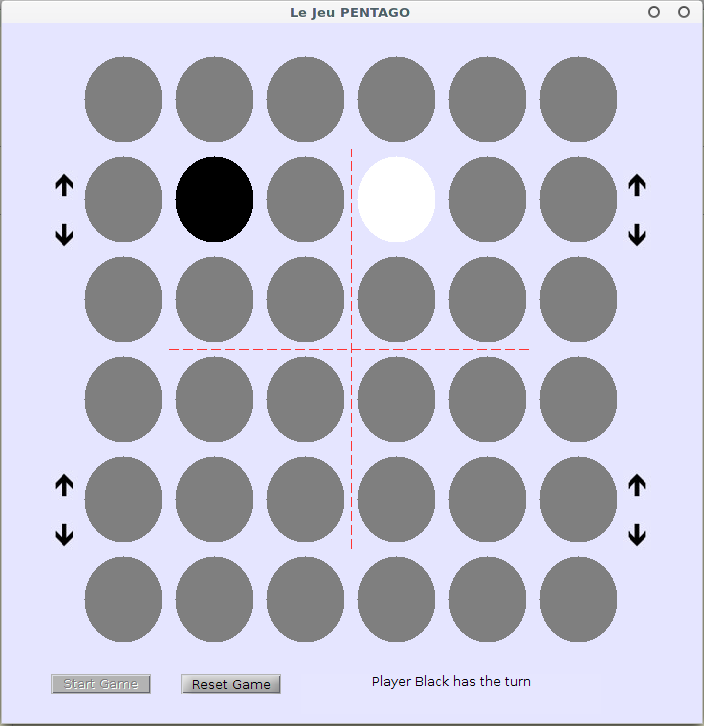
\includegraphics[scale=.25]{images/gui_jeu}
		\caption{The game's interface.}
		\label{fig:gui}
		\end{figure}

	\end{columns}

\end{frame}

\begin{frame}[fragile]

\frametitle{Graphical Interface - GUI}
\framesubtitle{Positioning of the components}

\begin{itemize}
  	\item Parameters of function \textbf{figure}:
	
	\begin{itemize}
	  
		\item \textbf{Visible}: determines whether the window will be visible or not.
		\item \textbf{Position}: an array containing the coordinates x and y of
		the screen, width and height of the window, respectively.
		\item \textbf{Name}: the string that will be displayed in the figure window.
		\item \textbf{Number Title}: this property set to \textit{off} means that the string
		\textit{Figure No} will not be displayed in the figure window.
		\item \textbf{Resize}: set to \textit{off} means that the window cannot be
		resized.
		\item \textbf{Color}: sets the background color of the figure. The array
		contains three values, which determine the color according to the
		(\textbf{R}ed, \textbf{G}reen, \textbf{B}lue) scale.

	\end{itemize}
	\item Example:
\begin{lstlisting}[language=Matlab]
plateau = figure ('Visible', 'on', 
	'Position', [1500, 1000, width, height], 
	'Name','Le Jeu PENTAGO',
	'NumberTitle','off', 'Resize', 'off',
	'Color', [0.9, 0.9, 1], 'MenuBar', 'none');
\end{lstlisting}
\end{itemize}

\end{frame}

\begin{frame}[fragile]
\frametitle{Graphical Interface - GUI}
\framesubtitle{Positioning of the components}

\begin{itemize}
  	\item Parameters of function \textbf{uicontrol}:
	
	\begin{itemize}
	  
		\item \textbf{Callback}: It specifies a function handler, which will be
		activated when the button is pressed. \\
\begin{lstlisting}[language=Matlab]
buttonStart = uicontrol ('Position', [50 30 100 20], 'String', 'Start Game','Callback', @start_pressed);
\end{lstlisting}
	\end{itemize}
	
	
	\item Parameters of the function \textbf{image}:
	
	\begin{itemize}
	  
		\item \textbf{ButtonDownFcn}: equivalent to the property \textbf{Callback}
		detailed previously. 
		\item Function \textbf{imread(\ldots)}: reads an image from specified file.
\begin{lstlisting}[language=Matlab]
rotate_up = imread('arrow_alt_up.jpeg');
textQ1R   = image(-30,400,rotate_up, 'ButtonDownFcn',{@turn_pressed, 1, 'L'});
\end{lstlisting}
	\end{itemize}
	
\end{itemize}
\end{frame}


\begin{frame}[fragile]

\frametitle{Graphical Interface - GUI}
\framesubtitle{Positioning of the components}
	\begin{columns}
	\column{0.5\textwidth}
		
		\begin {itemize}
		\item Parameters of the function  \textbf{axes}:
	
	\begin{itemize}
	  
 
		\item \textbf{Color}: specify the color of the axes back planes. Setting it to
		\textit{none} means that the axes is transparent and the figure color shows through
		\item \textbf{Visible}: component's visibility. Setting it to
		\textit{off} prevents axis lines, tick marks, and labels from being displayed.\\
\begin{lstlisting}[language=Matlab]
axes1 = axes([...],'Color', 'none', 'Visible', 'off');
\end{lstlisting}

	\end{itemize}
	\end{itemize}
		
	\column{0.5\textwidth}
		\begin{figure}[h]
		\centering
		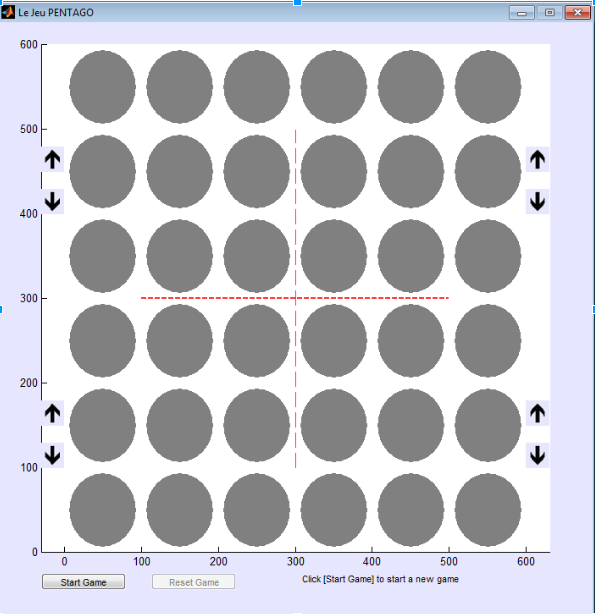
\includegraphics[scale=.30]{images/noeffects}
		\caption{\textit{Axis1} with \textit{Color} and \textit{Visible} 
different from \textit{none} and \textit{off}}
		\label{fig:noeffects}
		\end{figure}

	\end{columns}

\end{frame}


\begin{frame}
\frametitle{Graphical Interface - GUI}
\framesubtitle{Evaluating a board}

\begin{itemize}
  \item Les variables utilisées:
  
	\begin{itemize}
	 
	  	\item \textbf{value}: the result that will be given to that board.
		\item Each element of \textbf{hasBeenDetected} is an integer whose
		representation in binary determines if that element has already been detected 
		taking place in at least one line/column or diagonal.
		\item \textbf{playerScores}: an array that stores the scores of all 
		combination the player’s got so far in each one of the possible configurations.
		\item \textbf{opponentScores}: is the same that \textit{playerScores} but for
		the opponent.
		\item \textbf{foundUltraCondition} is true if we detect a line, column or 
		diagonal completely filled with 5 pieces.
	
	 	 
	\end{itemize}
\end{itemize}

\end{frame}

\begin{frame} [fragile]
\frametitle{Graphical Interface - GUI}
\framesubtitle{Evaluating a board}

\begin{itemize}
  \item Example, checking the lines for a row:\\
\begin{lstlisting} [basicstyle=\tiny\ttfamily, numberstyle={\tiny
\color{black}}] 
while (offset_index >= 1) && (bitand(hasBeenDetected(x,y), 2) == 0) && ...
        (foundUltraCondition == 0)
    
    if (y + offset_index) <= 6
        t = state_matrix (x , y:(y + offset_index));
        
        if all(t == t(1))
           
            if offset_index == 4
                foundUltraCondition = 1;
            end
            
            scores(2, index_player) = scores(2, index_player) + 10^(3*(offset_index+1));
           
            hasBeenDetected (x , y:(y + offset_index)) = ...
                hasBeenDetected (x , y:(y + offset_index)) + 2;
            
        elseif offset_index == 4
            
            if (sum (t == player) == 4) && (sum (t == opponent) == 1)
                value = value + 10^14;
            elseif (sum (t == player) == 1) && (sum (t == opponent) == 4)
                value = value - 10^14;
            end
            
        end   
    end
    offset_index = offset_index - 1;
end
\end{lstlisting}
  
\end{itemize}
\end{frame}

%==================================================================================================

\subsection{PENTAGO's algorithm}
\begin{frame}
\frametitle{PENTAGO's algorithm}
\framesubtitle{The choice of the algorithm}

	\begin{itemize}
	  
		\item Computational resources constraints: processing time and memory.
		
			\begin{itemize}
			  \item Search algorithms with acceptable complexity instead of full search.
			  	\begin{itemize}
			  	  \item Ex.: Alpha-beta, Proof-number, Threat-space, Retrograde.
			  	  \item Most employed and our choice: Alpha-beta search
			  	\end{itemize}
			\end{itemize}
			
		\item The Alpha-beta search:
		
			\begin{itemize}
			  
			  \item Based on the minimax algorithm.
			  \item Two players evaluate a function, one of them tries to maximize and to
			  the other to minimize it.
			  	\begin{itemize}
			  	  \item The value that will be achieve is:\\ 
			  	  \(\max \{ \min \{ \max \{ \min \ldots \max \{ \min \{ eval \} \} \} \}
			  	  \} \)
			  	\end{itemize}
			  
			  \item Pruning:
			    \begin{itemize}
			  	  \item If a branch cannot change the result, we skip its whole subtree. 
			  	\end{itemize}
			  
			\end{itemize}
				
	\end{itemize}
\end{frame}

%==================================================================================================
\begin{frame}
\frametitle{PENTAGO's algorithm}
\framesubtitle{Algorithm and complexity}

	\begin{itemize}
	  
		\item  Algorithm description:
		
			\begin{enumerate}
			  \item Consider a node n somewhere in the tree, such that one can move to
			  that node.
			  \item If there is a better choice m either at the parent of the node n or
			  at any choice point further up, n will never be reached.
			  \item Once we have enough information about n to reach this conclusion, we
			  can prune it.
			\end{enumerate}
			
		\item Complexity, by the arrange of the nodes (branching factor b, search
		depth d):
		
			\begin{itemize}
			  
			  \item Pessimal: \(\mathcal{O}(bd)\) - the same as the simple minimax.
			  \item Optimal: \(\mathcal{O} (\frac{bd}{2}) = \mathcal{O}( \sqrt {bd} ) \).
			  \item Random: \(\mathcal{O} ( b\frac{3d}{4})\).

			\end{itemize}
				
	\end{itemize}
\end{frame}

%==================================================================================================
\begin{frame}
\frametitle{PENTAGO's algorithm}
\framesubtitle{The pruning\ldots Alpha? Beta?}

	\begin{itemize}
	  
		\item  Alpha-Beta pruning gets its name from the following parameters:
		
			\begin{enumerate}
			  \item \(\alpha\) = the value of the best choice we have found so far at any
			  choice point along the path for MAX.
			  \item \(\beta\) = the value of the best choice we have found so far at any
			  choice point along the path for MIN.
			\end{enumerate}
			
		\item Alpha-Beta search:
		
			\begin{itemize}
			  
			  \item Updates the values of \(\alpha\) and \(\beta\) as it goes along.
			  \item Prunes the remaining branches at a node
			  \begin{itemize} 
				  \item As soon as the value of the current node is known to be worse than
				  the current values of \(\alpha\) and \(\beta\).
				  \item Therefore, it does not affect the solution.
			  \end{itemize}
			\end{itemize}
				
	\end{itemize}
\end{frame}

%==================================================================================================
\begin{frame}
\frametitle{PENTAGO's algorithm}
\framesubtitle{Demonstration - Video}

	\begin{itemize}
	  
		\item  Minimax - Alpha Beta Pruning (Artificial Intelligence) by Ice
		Blended. \\
		Available at: \url{https://youtu.be/SROIGH1P2No?t=104}. Start watching at
		1:45\\
		%\movie[(options)]{}{(lien vidéo)}
				
	\end{itemize}
\end{frame}

%==================================================================================================
\begin{frame}[fragile]

\frametitle{PENTAGO's algorithm}
\framesubtitle{Coding (1)}

\begin{itemize}
  	\item The function will return an array. This array will contain:
	
	\begin{itemize}
	  
		\item \textbf{eval\_value}: the evaluation of the board.
		\item \textbf{move}: the place (convention [line column]) where the next piece
		will be played
		\item \textbf{quadrant}: The quadrant where the rotation is applied after the
		piece be placed.

		\item \textbf{direction}: The direction of the rotation.

	\end{itemize}
	\item Example:
\begin{lstlisting}[language=Matlab]
function [eval_value move quadrant direction] = alpha_beta_search (state_matrix, emptySlots, depth, alpha, beta, isMaximizing, player)
\end{lstlisting}
\end{itemize}

\end{frame}

%==================================================================================================
\begin{frame}[fragile]

\frametitle{PENTAGO's algorithm}
\framesubtitle{Coding (2) - Variables and Recursion}

\begin{itemize}
  	\item Variables used in the search:
	
	\begin{itemize}
	  
		\item \textbf{alpha, beta}: Parameters of the Alpha-Beta search, said
		previously.
		\item \textbf{depth}: The depth left by the search. Starts at 2 goes to 0.
		\item \textbf{mustStop}: allows us to do the pruning. Do so by breaking the
		while loops that are used to explore our tree, thus skipping the subtree.

	\end{itemize}
	\item Recursive function:
	
	\begin{itemize}
	  
		\item Base case: maximum depth reached or no possible plays.\\
\begin{lstlisting}[language=Matlab]
if depth == 0 || emptySlots == 0
    [eval_value] = evaluate_board(state_matrix, player);
    move = []; quadrant = 0; direction = 0;
\end{lstlisting}
		\item Else: explore subtree.\\
\begin{lstlisting}[language=Matlab]
else   
    dir = ['L' 'R'];  mustStop = 0;
    if (isMaximizing == 1) eval_ = -inf;
    else eval_ = +inf;
    end
\end{lstlisting}
		
	\end{itemize}
\end{itemize}

\end{frame}

%==================================================================================================
\begin{frame}[fragile]

\frametitle{PENTAGO's algorithm}
\framesubtitle{Coding (3) - A cascade of loops}

\begin{itemize}
  	\item A cascade of while loops to emule a tree structure. The exploration
  	stops when we arrive to:
	
	\begin{itemize}
	  
		\item Natural limits of the 6x6 board.
		\item Pruned subtrees.

	\end{itemize}
	\item In our case:\\

\begin{lstlisting}[basicstyle=\tiny\ttfamily, numberstyle={\tiny
\color{black}}]
l = 1;
while (l <= 6) && (mustStop == 0)   
    c = 1;
    while (c <= 6) && (mustStop == 0)
        if state_matrix (l,c) == 0
            quad_index = 1;
            while (quad_index <=4) && (mustStop == 0)
                dir_index = 1;
                while (dir_index <= 2) && (mustStop == 0)
                    if isMaximizing == 1
                        state_matrix (l,c) = player;
                    else
                        if player == 'B'
                            state_matrix (l,c) = 'W';
                        else
                            state_matrix (l,c) = 'B';
                        end
                    end
                    state_matrix = rotate_quadrant (state_matrix, quad_index,
                    	 dir (dir_index) );
\end{lstlisting}
\end{itemize}

\end{frame}

%==================================================================================================
\begin{frame}[fragile]

\frametitle{PENTAGO's algorithm}
\framesubtitle{Coding (4) - Alpha-beta search coded}

\begin{itemize}
  	\item Implementation of the alpha-beta search algorithm.
	
	\begin{itemize}
	  
		\item Started as a pseudo code.

	\end{itemize}
 

\end{itemize}

\begin {columns}
\column{0.5\textwidth}
\begin{lstlisting}[basicstyle=\tiny\ttfamily, numbers=none]
state_game_ = verify_victory(state_matrix);
if isMaximizing == 1
    if state_game_ == player
        eval_MIN = +10^20;
        mustStop = 1;
    else
        [eval_MIN move_MIN quadrant_MIN direction_MIN] = ...
            alpha_beta_search(state_matrix, emptySlots - 1, depth - 1, alpha, beta, 0, player);                        
    end
    if eval_ < eval_MIN
        eval_ = eval_MIN; 
        eval_value = eval_;
        move = [l c]; 
        quadrant = quad_index;
        direction = dir (dir_index);
        
    end
    if eval_ >= beta
        mustStop = 1;
    end
    alpha = max(alpha, eval_)
\end{lstlisting}
		
	\column{0.5\textwidth}
\begin{lstlisting}[basicstyle=\tiny\ttfamily, numbers=none]
elseif isMaximizing == 0
    if (state_game_ ~= player) && (state_game_ ~= 0) && (state_game_ ~= 'D')
        eval_MAX = -10^20;
        mustStop = 1;
    else
        [eval_MAX move_MAX quadrant_MAX direction_MAX] = ...
            alpha_beta_search(state_matrix, emptySlots - 1, depth - 1, alpha, beta, 1, player);
    end
    if eval_ > eval_MAX 
        eval_ = eval_MAX; 
        eval_value = eval_;
        move = [l c]; 
        quadrant = quad_index;
        direction = dir (dir_index);
  	end
    if alpha >= eval_
        mustStop = 1;
    end
    beta  = min(beta, eval_);
\end{lstlisting}

\end{columns}

\end{frame}

%==================================================================================================
\begin{frame}[fragile]

\frametitle{PENTAGO's algorithm}
\framesubtitle{Coding (5) - End of an iteration}

\begin{itemize}
  	\item Restore the state of our board(state\_matrix) to how it was before
  	doing the play that we are analysing
	
	\begin{itemize}
	  
		\item Achieved by doing the reverse of all modifications that we have applied
		since we ran the alpha beta search on the board.

	\end{itemize}
	
	\item Update loop parameters and start another iteration.\\

\begin{lstlisting}[language=Matlab]
	if dir (dir_index) == 'L'
		state_matrix = rotate_quadrant(state_matrix, quad_index, 'R');
	else
		state_matrix = rotate_quadrant(state_matrix, quad_index, 'L');
	end

	state_matrix (l,c) = 0;
	dir_index = dir_index + 1;
end
quad_index = quad_index + 1;
end
\end{lstlisting}
\end{itemize}

\end{frame}

%==================================================================================================
\subsection{Battle of AIs - A statistical point of view}

\begin{frame}
\frametitle{Battle of AIs - A statistical point of view}
\framesubtitle{Simulation}

	\begin{columns}
	\column{0.5\textwidth}
		
		\begin{itemize}
		  \item Player \textbf{Black} represents your artificial intelligence.
		  \item Player \textbf{White} represents ours.
		  \item 500 matches simulated: 
		
			\begin{itemize}
			  \item Each AI has the first move in exactly half of them, that is, 250 matches.
			  \item 193 (90 of them when it started playing) were won by player
			  \textbf{White}.
			  \item 223 (116  of them when it started playing) were won by player
			  \textbf{Black}.
			  \item 84 (44 when \textbf{Black} started) resulted in draws. 
			  
			\end{itemize}
	
		\end{itemize}
		
	\column{0.5\textwidth}
		\begin{figure}[h]
		\centering
		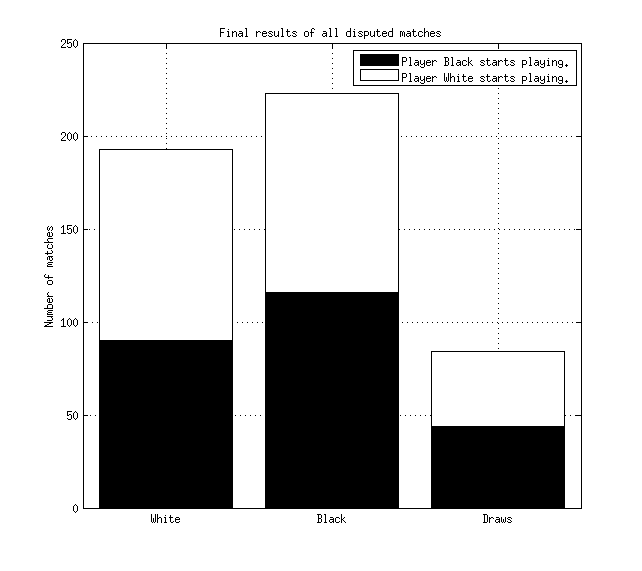
\includegraphics[scale=.3 ]{images/victories_count}
		\caption{\centering Number of victories of each player.}
		\label{fig:gui}
		\end{figure}

	\end{columns}
\end{frame}

%=============================================================================================================

\begin{frame}
\frametitle{Battle of AIs - A statistical point of view}
\framesubtitle{Some probabilities}

\begin{itemize}
  	\item Based on the previous results, we can observe that:
	
	\begin{itemize}
	  \item For player \textbf{Black}: \\
	  	 \(\mathrm{P}(\textbf{B})= \frac{223}{500} = 0.446  \) \\
	  	 \(\mathrm{P}(\textbf{B} \mid  \textbf{B}_{started})= \frac{116}{250} =
	  	 0.464  \)\\
	  	 \(\mathrm{P}(\textbf{B} \mid  \textbf{W}_{started})=
	  	 \frac{107}{250} = 0.428  \)
	  	 
	  	 \vspace{10pt}
	 \item For player \textbf{White}: \\
	  	 \(\mathrm{P}(\textbf{W})= \frac{193}{500} = 0.386  \) \\
	  	 \(\mathrm{P}(\textbf{W} \mid  \textbf{B}_{started})= \frac{90}{250} =
	  	 0.360  \)\\
	  	 \(\mathrm{P}(\textbf{W} \mid  \textbf{W}_{started})=
	  	 \frac{103}{250} = 0.412  \) 
	  	 
	  	 \vspace{10pt}
	\item In case of \textbf{match nul}: \\
	  	 \(\mathrm{P}(\textbf{M}_{draw})= \frac{84}{500} = 0.168  \) \\
	  	 \(\mathrm{P}(\textbf{M}_{draw} \mid  \textbf{B}_{started})= \frac{44}{250}
	  	 = 0.176  \)\\
	  	 \(\mathrm{P}(\textbf{M}_{draw} \mid  \textbf{W}_{started})=
	  	 \frac{40}{250} = 0.160  \)

	\end{itemize}
\end{itemize}
\end{frame}

%=============================================================================================================

\begin{frame}
\frametitle{Battle of AIs - A statistical point of view}
\framesubtitle{Decision time for each player}

	\begin{columns}
	\column{0.5\textwidth}
		
		\begin{itemize}
		  
		  \item Player \textbf{Black} takes, in average, \textbf{2.05}
		  seconds to decide.
	
		\end{itemize}
		
		\vspace{-15pt}
		
		\begin{figure}[h]
		\centering
		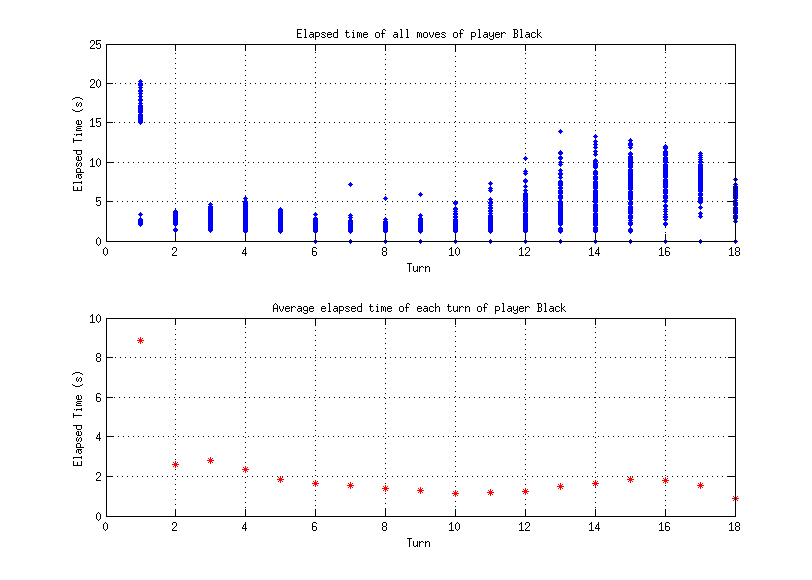
\includegraphics[scale=.22 ]{images/LBtimes}
		\caption{\centering Required time to Player \textbf{Black} take a move.}
		\label{fig:gui}
		\end{figure}
		
		
	\column{0.5\textwidth}
	
		\begin{itemize}
			\item Player \textbf{White} takes, in average, \textbf{9.5}  seconds to
			decide.
		\end{itemize}
		
		\vspace{-25pt}
		
		\begin{figure}[h]
		\centering
		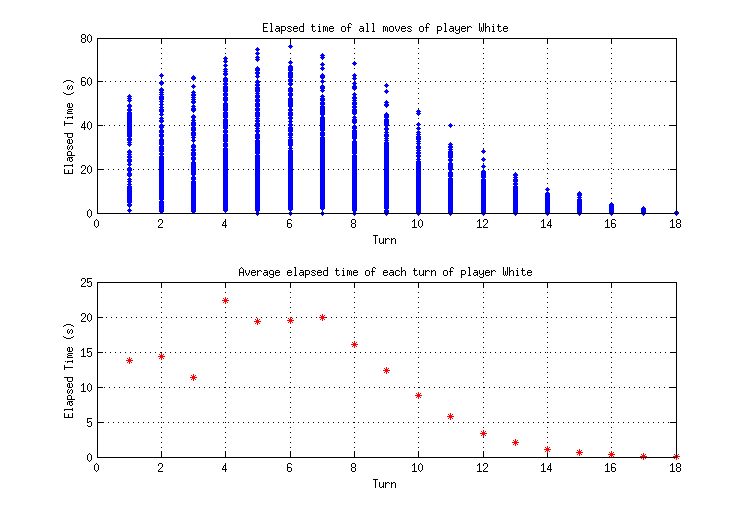
\includegraphics[scale=.26 ]{images/PENTAGOtimes}
		\caption{\centering Required time to Player \textbf{White} take a move.}
		\label{fig:gui}
		\end{figure}

	\end{columns}
\end{frame}

%=============================================================================================================
\begin{frame}
\frametitle{Battle of AIs - A statistical point of view}
\framesubtitle{Comparison of algorithms}

	\begin{itemize}
		
		\item The difference between these two times is explained by how which  
		algorithm decides the move and evaluates a board.
		  
		\begin{itemize}
			\item Our algorithm needs to verify each position of the matrix at least
			twice: once to evaluate if that \textbf{position belongs to a row, column or
			diagonal}, and another to conclude if that \textbf{move is profitable}.
		\end{itemize} 
		  
		
		 \item The \textbf{first eight moves} of player \textbf{White} take almost
		 \textbf{all the time of decision}.\\
		  That’s already expected: at the beginning of the  match, there are more
		  positions to be verified, contrarily to the end, in which few available
		  positions remain.
	
		\item Player \textbf{Black}'s moves takes roughly constant time, around 2
		seconds, to be decided. The only move that does not follow that property is the first one.
		 
	\end{itemize}


\end{frame}


%=============================================================================================================
\section{Conclusion}
\begin{frame}
\frametitle{Conclusion}

	\begin{itemize}
		
		\item Obtained results:
		  
		\begin{itemize}
			\item Graphical interface: Easy to use, functional and enjoyable.
			\item AI:
			\begin{itemize}
			  \item Human vs Human, AI vs AI and mixed matches enabled.
			  \item Good performance: Comparable with the one of our advisor.
			\end{itemize}
		\end{itemize} 
		  
		
		 \item Room for improvement (some of them may be beyond a 2 month project!):
		 	\begin{itemize}
			  \item Programming Language: C++ instead of Matlab.
			  \item Algorithm: Transition tables, deeper search.
			  \item Hardware: GPU processing, supercomputers.
		 	\end{itemize}
		 	
	
		\item Aftermatch
		 	\begin{itemize}
			  \item The next generation of students may take from where we left and
			  pursuit one of the lines of improvement.
			  \item Or simply have our algorithm as a reference, as we had Mr.
			  Bourgois'.
		 	\end{itemize}
		 
	\end{itemize}
\end{frame}

%=============================================================================================================
\section{Bibliography}

\begin{frame}[fragile]
\frametitle{Bibliography (1)}

	\begin{itemize}
	\item Pentago, (2015). Pentago. [online] Available at:\\
	\url{http://en.wikipedia.org/wiki/Pentago} [Accessed 14 Apr. 2015].

	\item Pentago is a first player win, (2015). [online] Available at:\\
	\url{https://perfect-pentago.net/details.html#intro} [Accessed 14 Apr. 2015].

	\item On solving Pentago, (2015). [online] Available at:\\
	\url{http://www.ke.tu-darmstadt.de/lehre/arbeiten/bachelor/2011/Buescher_Niklas.pdf} [Accessed 14 Apr. 2015].

	\item Standford University, (2015).  [online] Available at:\\
	\url{http://web.stanford.edu/~msirota/soco/alphabeta.html} [Accessed 14 Apr.
	2015].
	
	\item Élagage alpha-beta, (2015).  [online] Available at:
	\url{http://fr.wikipedia.org/wiki/%C3%89lagage_alpha-beta} [Accessed 14 Apr. 2015].
	
	\end{itemize}
\end{frame}

\begin{frame} [fragile]
\frametitle{Bibliography (2)}

	\begin{itemize}
	
	\item Chalmers - GÖTEBORGS UNIVERSITET, (2015). [online] Available at:  
	\url{http://www.cse.chalmers.se/edu/year/2014/course/TIN172/example-exam-solutions.html}
	[Accessed 14 Apr. 2015].

	\item McCarthy, 2006. McCarthy, John (LaTeX2HTML 27 November 2006). "Human
	Level AI Is Harder Than It Seemed in 1955".
	\url{http://www-formal.stanford.edu/jmc/slides/wrong/wrong-sli/wrong-sli.html}
	[Acessed 20 Dec. 2006]

	\item Russell, Stuart J., 2003. Russell, Stuart J.; Norvig, Peter (2003),
	Artificial Intelligence: A Modern Approach (2nd ed.), Upper Saddle River, New
	Jersey: Prentice Hall, ISBN 0-13-790395-2  \url{http://aima.cs.berkeley.edu/}

	\item Nersc, (2015). [online] Available at:
	\url{https://www.nersc.gov/users/computational-systems/edison} [Accessed 19 May
	2015].

	\item NVIDIA, (2015). [online] Available at:
	\url{https://developer.nvidia.com/how-to-cuda-c-cpp} [Accessed 19 May 2015].
	
	\end{itemize}
\end{frame}

\end{document}
